\chapter{管道与Shell}
%目标:user/pipe.c 与 user/sh.c
%是否新增?
%是否需要自行编写测试文件?/个人觉得这里应该要求自己编写测试文件进行测试(说明白原理即可)
\section{实验目的}
\begin{enumerate}
	\item 掌握管道的原理与底层细节
	\item 实现管道的读写
	\item 复述管道竞争情景
	\item 实现shell中涉及管道的部分
\end{enumerate}

\section{管道}

在lab4中,我们已经学习过一种进程间通信(IPC,Inter-Process Communication)的方式——共享内存。
而今天我们要学的管道,其实也是进程间通信的一种方式。

\subsection{初窥管道}

通俗来讲,管道就像家里的自来水管:一端用于注入水,一端用于放出水,且水只能在一个方向上流动,而不能双向流动,所以说管道是典型的单向通信。管道又叫做匿名管道,只能用在具有公共祖先的进程之间使用,通常使用在父子进程之间通信。
 
在Unix中,管道由pipe函数创建,函数原型如下:

\begin{minted}[linenos]{c}
	#include<unistd.h>
	
	int  pipe(int fd[2]); 成功返回0,否则返回-1;
	
	参数fd返回两个文件描述符,fd[0]对应读端,fd[1]对应写端。
\end{minted}

为了更好地理解管道实现的原理,同样,我们先来做实验亲自体会一下\footnote{实验代码参考 http://pubs.opengroup.org/onlinepubs/9699919799/functions/pipe.html}

\begin{codeBoxWithCaption}{管道示例\label{code:test_pipe.c}}
	\inputminted[linenos]{c}{codes/test_pipe.c}
\end{codeBoxWithCaption}

示例代码实现了从父进程向子进程发送消息"Hello,world",并且在子进程中打印到屏幕上。它演示了管道在父子进程之间通信的基本用法:在pipe函数之后,调用fork来产生一个子进程,之后在父子进程中执行不同的操作。在示例代码中,父进程操作写端,而子进程操作读端。同时,示例代码也为我们演示了使用pipe系统调用的习惯:fork之后,进程在开始读或写管道之前都会关掉不会用到的管道端。

从本质上说,管道是一种只在内存中的文件。在UNIX中使用pipe系统调用时,进程中会打开两个新的文件描述符:一个只读端和一个只写端,而这两个文件描述符都映射到了同一片内存区域。但这样建立的管道的两端都在同一进程中,而且构建出的管道两端是两个匿名的文件描述符,这就让其他进程无法连接该管道。在fork的配合下,才能在父子进程间建立起进程间通信管道,这也是匿名管道只能在具有亲缘关系的进程间通信的原因。

\begin{thinking}\label{think-father-reader}
	示例代码中,父进程操作管道的写端,子进程操作管道的读端。如果现在想让父进程作为“读者”,代码应当如何修改?
\end{thinking}

\subsection{管道的测试}

我们下面就来填充函数实现匿名管道的功能。思考刚才的代码样例,要实现匿名管道,至少需要有两个功能:管道读取、管道写入。

要想实现管道,首先我们来看看本次实验我们将如何测试。lab6关于管道的测试有两个,分别是\mintinline{console}|user/testpipe.c|与\mintinline{console}|user/testpiperace.c|。

首先我们来观察testpipe的内容

\begin{codeBoxWithCaption}{testpipe测试\label{code:lab_test_pipe.c}}
	\inputminted[linenos]{c}{codes/lab_test_pipe.c}
\end{codeBoxWithCaption}

实际上可以看出,测试文件使用pipe的流程和示例代码是一致的。先使用函数 \mintinline{c}|pipe(int p[2]) |创建了管道,读端的文件控制块编号\footnote{文件控制块编号是int型,user/fd.c 中 num2fd 函数可通过它定位文件控制块的地址。}为p[0],写端的文件控制块编号为p[1]。之后使用fork()创建子进程,\textbf{注意这时父子进程使用p[0]和p[1]访问到的内存区域一致}。之后子进程关闭了p[1],从p[0]读;父进程关闭了p[0],从p[1]写入管道。

lab4的实验中,我们的fork实现是完全遵循Copy-On-Write原则的,即对于所有用户态的地址空间都进行了PTE\_COW的设置。
但实际上写时复制并不完全适用,至少在我们当前情景下是不允许写时拷贝。为什么呢?我们来看看pipe函数中的关键部分就能知晓答案:

\begin{minted}[linenos]{c}
int
pipe(int pfd[2])
{
	int r, va;
	struct Fd *fd0, *fd1;
	
	if ((r = fd_alloc(&fd0)) < 0
	||  (r = syscall_mem_alloc(0, (u_int)fd0, PTE_V|PTE_R|PTE_LIBRARY)) < 0)
	goto err;
	
	if ((r = fd_alloc(&fd1)) < 0
	||  (r = syscall_mem_alloc(0, (u_int)fd1, PTE_V|PTE_R|PTE_LIBRARY)) < 0)
	goto err1;
	
	va = fd2data(fd0);
	if ((r = syscall_mem_alloc(0, va, PTE_V|PTE_R|PTE_LIBRARY)) < 0)
	goto err2;
	if ((r = syscall_mem_map(0, va, 0, fd2data(fd1), PTE_V|PTE_R|PTE_LIBRARY)) < 0)
	goto err3;
	
	...
}
\end{minted}

在pipe中,首先分配两个文件描述符并为其分配空间,然后将一个管道作为这两个文件描述符数据区的第一页数据,从而使得这两个文件描述符能够共享一个管道的数据缓冲区。

\begin{exercise}
	仔细观察pipe中新出现的权限位\mintinline{c}|PTE_LIBRARY|,根据上述提示修改fork系统调用,使得\textbf{管道缓冲区是父子进程共享的},不设置为写时复制的模式。
\end{exercise}

下面我们使用一张图来表示父子进程与管道的数据缓冲区的关系:

\begin{figure}[htbp]
	\centering
	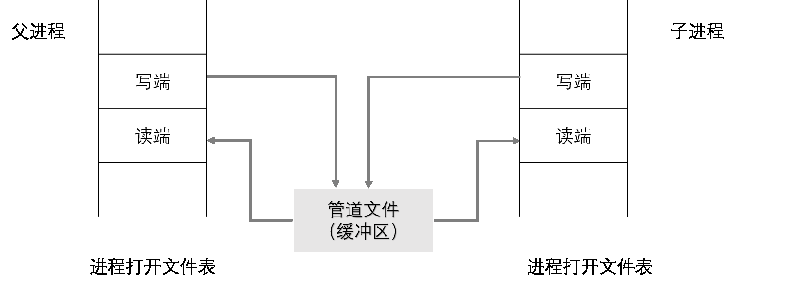
\includegraphics[width=15cm]{6-pipe-after-fork}
	\caption{父子进程与管道缓冲区}\label{fig:6-pipe-after-fork} 
\end{figure}

实际上,在父子进程中各自close掉不再使用的端口后,父子进程与管道缓冲区的关系如下图:

\begin{figure}[htbp]
	\centering
	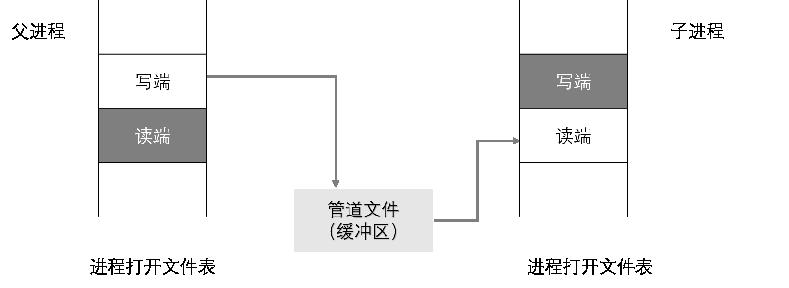
\includegraphics[width=15cm]{6-pipe-after-close}
	\caption{关闭不使用的端口后}\label{fig:6-pipe-after-close} 
\end{figure}

下面我们来讲一下\mintinline{c}|struct Pipe|,并开始着手填写操作管道端的函数。

\subsection{管道的读写}

我们可以在 user/pipe.c 中轻松地找到Pipe结构体的定义,它的定义如下:

\begin{minted}[linenos]{c}
	struct Pipe {
		u_int p_rpos;		    // read position
		u_int p_wpos;		    // write position
		u_char p_buf[BY2PIPE];	// data buffer
	};
\end{minted}

在Pipe结构体中,p\_rpos给出了下一个将要从管道读的数据的位置,而p\_wpos给出了下一个将要向管道写的数据的位置。只有读者可以更新p\_rpos,同样,只有写者可以更新p\_wpos,读者和写者通过这两个变量的值进行协调读写。一个管道有BY2PIPE(32Byte)大小的缓冲区。

这个只有BY2PIPE大小的缓冲区发挥的作用类似于环形缓冲区,所以下一个要读或写的位置i实际上是i\%BY2PIPE。

读者在从管道读取数据时,要将p\_buf[p\_rpos\%BY2PIPE]的数据拷贝走,然后读指针自增1。但是需要注意的是,管道的缓冲区此时可能还没有被写入数据。所以如果管道数据为空,即当 p\_rpos >= p\_wpos时,应该进程切换到写者运行。

类似于读者,写者在向管道写入数据时,也是将数据存入p\_buf[p\_wpos\%BY2PIPE],然后写指针自增1。 需要注意管道的缓冲区可能出现满溢的情况,所以写者必须得在 p\_wpos - p\_rpos < BY2PIPE时方可运行,否则要一直挂起。

上面这些还不足以使得读者写者一定能顺利完成管道操作。假设这样的情景:管道写端已经全部关闭,读者读到缓冲区有效数据的末尾,此时有 p\_rpos = p\_wpos。按照上面的做法,我们这里应当切换到写者运行。但写者进程已经结束,进程切换就造成了死循环,这时候读者进程如何知道应当退出了呢?

为了解决上面提出的问题,我们必须得知道管道的另一端是否已经关闭。不论是在读者还是在写者中,我们都需要对另一端的状态进行判断:当出现缓冲区空或满的情况时,要根据另一端是否关闭来判断是否要返回。如果另一端已经关闭,进程返回0即可;如果没有关闭,则切换到其他进程运行。

\begin{note}
Unix : If all file descriptors referring to the write end of a pipe have been closed, then an attempt to read(2) from the pipe will see end-of-file (read(2) will return 0) link : http://linux.die.net/man/7/pipe
\end{note}

那么我们该如何知晓管道的另一端是否已经关闭了呢?这时就要用到我们的\mintinline{c}|static int _pipeisclosed(struct Fd *fd, struct Pipe *p)|函数。而这个函数的核心,就是下面我们要讲的恒成立等式了。

在之前的图\ref{fig:6-pipe-after-close}中我们没有明确画出文件描述符所占的页,但实际上,对于每一个匿名管道而言,我们分配了三页空间:一页是读数据的文件描述符rfd,一页是写数据的文件描述符wfd,剩下一页是被两个文件描述符共享的管道数据缓冲区。既然管道数据缓冲区h是被两个文件描述符所共享的,我们很直观地就能得到一个结论:如果有1个读者,1个写者,那么管道将被引用2次,就如同上图所示。pageref函数能得到页的引用次数,所以实际上有下面这个等式成立:

pageref(rfd) + pageref(wfd) = pageref(pipe)\label{variant}

\begin{note}
内核会对pages数组成员维护一个页引用变量 pp\_ref 来记录指向该物理页的虚页数量。pageref的实现实际上就是查询虚页 P 对应的实际物理页,然后返回其 pp\_ref 变量的值。
\end{note}

这个等式对我们而言有什么用呢?假设我们现在在运行读者进程,而进行管道写入的进程都已经结束了,那么此时就应该有:\mintinline{c}|pageref(wfd) = 0|。所以就有\mintinline{c}|pageref(rfd) = pageref(pipe)|。所以我们只要判断这个等式是否成绩就可以得知写端是否关闭,对写者来说同理。

\begin{exercise}
	根据上述提示与代码中的注释,填写 user/pipe.c 中的 piperead、pipewrite、\_pipeisclosed 函数并通过 testpipe 的测试。
\end{exercise}

\begin{note}
注意在本次实验中由于文件系统服务所在进程已经默认为1号进程(起始进程为0号进程),在测试时想启用文件系统需要注意ENV\_CREATE(fs\_serv) 在 init.c 中的位置。
\end{note}

\subsection{管道的竞争}

我们的小操作系统采用的是时间片轮转调度的进程调度算法,这点你应该在lab3中就深有体会了。这种抢占式的进程管理就意味着,用户进程随时有可能会被打断。

当然,如果进程间是孤立的,随时打断也没有关系。但当多个进程共享同一个变量时,执行同一段代码,不同的进程执行顺序有可能产生完全不同的结果,造成运行结果的不确定性。而进程通信需要共享(不论是管道还是共享内存),所以我们要对进程中共享变量的读写操作有足够高的警惕。

实际上,因为管道本身的共享性质,所以在管道中有一系列的竞争情况。在当前这种不加锁控制的情况下,我们无法保证\mintinline{c}|_pipeisclosed|用于管道另一端关闭的判断一定返回正确的结果。

我们重新看之前写的\mintinline{c}|_pipeisclosed|函数。在这个函数中我们对\mintinline{c}|pageref(fd structure)|与 
\mintinline{c}|pageref(pipe structure)|进行了等价关系的判断。假如不考虑进程竞争,不论是在读者还是写者进程中,我们会认为:

\begin{itemize}
	\item 对fd和对pipe的pp\_ref 的\textbf{写入}是同步的。
	\item 对fd和对pipe的pp\_ref 的\textbf{读取}是同步的。 
\end{itemize}

但现在我们处于进程竞争、执行顺序不定的情景下,上述两种情况现在都会出现不同步的现象。想想看,如果在下面这种场景下,我们前面提到的等式\ref{variant}还是恒成立的吗:

\label{code:example-pipe}
\begin{minted}[linenos]{c}
	pipe(p);
	if(fork() == 0 ){
		close(p[1]);
		read(p[0],buf,sizeof buf);
	}else{
		close(p[0]);
		write(p[1],"Hello",5);
	}
\end{minted}

\begin{itemize}
	\item  fork结束后,子进程先执行。时钟中断产生在close(p[1])与read之间,父进程开始执行。
	\item 父进程在close(p[0])中,p[0]已经解除了对pipe的映射(unmap),还没有来得及解除对p[0]的映射,时钟中断产生,子进程接着执行。
	\item 注意此时各个页的引用情况: pageref(p[0]) = 2(因为父进程还没有解除对p[0]的映射),而pageref(p[1]) = 1(因为子进程已经关闭了p[1])。但注意,此时pipe的pageref是2,子进程中p[0]引用了pipe,同时父进程中p[0]刚解除对pipe的映射,所以在父进程中也只有p[1]引用了pipe。
	\item 子进程执行read,read中首先判断写者是否关闭。比较pageref(pipe)与pageref(p[0])之后发现它们都是2,说明写端已经关闭,于是子进程退出。
\end{itemize}

\begin{thinking}\label{think-dup}
	上面这种不同步修改pp\_ref而导致的进程竞争问题在 user/fd.c 中的dup函数中也存在。请结合代码模仿上述情景,分析一下我们的dup函数中为什么会出现预想之外的情况?
\end{thinking}

%问题的答案也简单,实际上是在dup函数的两次map之间,正确的顺序应该是先unmap fd,再unmap pipe。

那看到这里你有可能会问:在close中,既然问题出现在两次unmap之间,那么我们为什么不能使两次unmap统一起来是一个原子操作呢?要注意,在我们的小操作系统中,只有syscall\_开头的\textbf{系统调用函数}是原子操作,其他所有包括fork这些函数%\footnote{这里我们提到fork是“库函数”,好像与Linux里对fork是系统调用的措辞是矛盾的。但笔者认为,在我们的小操作系统中fork不算是系统调用。如果你持反对意见可以在报告中提出来。}
都是可能会被打断的。一次系统调用只能unmap一页,所以我们是不能保持两次unmap为一个原子操作的。那是不是一定要两次unmap是原子操作才能使得\mintinline{c}|_pipeisclosed|一定返回正确结果呢?

\begin{thinking}\label{think-automatic}
	阅读上述材料并思考:为什么系统调用一定是原子操作呢?如果你觉得不是所有的系统调用都是原子操作,请给出反例。希望能结合相关代码进行分析。
\end{thinking}

答案当然是否定的,\mintinline{c}|_pipeisclosed|函数返回正确结果的条件其实只是:

\begin{itemize}
	\item 写端关闭 当且仅当 pageref(p[0]) == pageref(pipe);
	\item 读端关闭 当且仅当 pageref(p[1]) == pageref(pipe);
\end{itemize}

比如说第一个条件,写端关闭时,当然有pageref(p[0]) == pageref(pipe)。所以我们要解决的实际上是 \textbf{当 pageref(p[0]) == pageref(pipe) 时,写端关闭}。正面如果不好解决 问题,我们可以考虑从其逆否命题着手,即要满足:{ 当写端没有关闭的时候, pageref(p[0]) $\neq$ pageref(pipe)}。

我们考虑之前那个预想之外的情景,它出现的最关键原因在于:pipe的引用次数总比fd要高。当管道的close进行到一半时,\textbf{若先解除pipe的映射,再解除fd的映射},就会使得pipe的引用次数的-1先于fd。这就导致在两个unmap的间隙,会出现pageref(pipe) == pageref(fd)的情况。那么若调换fd和pipe在close中的unmap顺序,能否解决这个问题呢?

\begin{thinking}\label{think-race}
	仔细阅读上面这段话,并思考下列问题
	\begin{itemize}
		\item 
		按照上述说法控制\textbf{pipeclose}中fd和pipe unmap的顺序,是否可以解决上述场景的进程竞争问题?给出你的分析过程。
		\item
		我们只分析了close时的情形,那么对于dup中出现的情况又该如何解决?请模仿上述材料写写你的理解。
	\end{itemize}
\end{thinking}

根据上面的描述我们其实已经能够得出一个结论:控制fd与pipe的map/unmap的顺序可以解决上述情景中出现的进程竞争问题。

那么下面根据你所思考的内容进行实践吧:

\begin{exercise}
	修改 user/pipe.c 中的 pipeclose 与 user/fd.c 中的 dup 函数 以避免上述情景中的进程竞争情况。
\end{exercise}

我们通过控制修改pp\_ref的前后顺序避免了“写数据”导致的错觉,但是我们还得解决第二个问题:
读取pp\_ref的同步问题。

同样是上面的代码\ref{code:example-pipe},我们思考下面的情景:

\begin{itemize}
	\item fork结束后,子进程先执行。执行完close(p[1])后,执行read,要从p[0]读取数据。但由于此时管道数据缓冲区为空,所以read函数要判断父进程中的写端是否关闭,进入到\_pipeisclosed函数,pageref(fd)值为2(父进程和子进程都打开了p[0]),时钟中断产生。
	\item 内核切换到父进程执行,父进程close(p[0]),之后向管道缓冲区写数据。要写的数据较多,写到一半时钟中断产生,内核切换到子进程运行。
	\item 子进程继续运行,获取到pageref(pipe)值为2(父进程打开了p[1],子进程打开了p[0]),引用值相等,于是认为父进程的写端已经关闭,子进程退出。
\end{itemize}

上述现象出现的根源在哪里呢?fd是一个父子进程共享的变量,但子进程中的pageref(fd)没有随父进程对fd的修改而同步,这就造成了子进程读到的pageref(fd)成为了“脏数据”。为了保证读的同步性,子进程应当重新读取pageref(fd)和pageref(pipe),并且要在\textbf{确认两次读取之间进程没有切换}后,才能返回正确的结果。为了实现这一点,我们要使用到之前一直都没用到的变量:env\_runs。

env\_runs记录了一个进程env\_run的次数,这样我们就可以根据某个操作do()前后进程env\_runs值是否相等,来判断在do()中进程是否发生了切换。

\begin{exercise}
	根据上面的表述,修改\mintinline{c}|_pipeisclosed|函数,使得它满足“同步读”的要求。注意env\_runs变量是需要维护的。
\end{exercise}

\section{shell}

shell本质上也是一个用户进程。它解释shell命令的工作是通过创建并运行子进程来完成的:对于每个shell命令,都有一个对应的可执行文件来完成该命令所要完成的工作,shell需要根据所得到的命令来创建执行相应可执行文件的子进程,从而完成命令的解释工作并得到结果。

为了能够使用shell,首先需要使我们的操作系统响应键盘的输入,让shell能够获得用户输入的命令。我们已经使用汇编完成了sys\_cgetc函数,你可以在 lib/getc.S 中看到它的具体实现。但是光有sys\_cgetc函数还不够,你需要增加系统调用syscall\_cgetc来获取键盘的输入。

\begin{exercise}
	模仿现有的系统调用,增加系统调用syscall\_cgetc。(提示:sys\_cgetc函数不需要传入参数)
\end{exercise}

接下来,我们需要在shell进程里实现对管道和重定向的解释功能。解释shell命令时:

\begin{enumerate}
	\item 如果碰到重定向符号‘<’或者’>’,则读下一个单词,打开这个单词所代表的文件,然后将其复制给标准输入或者标准输出。
	\item 如果碰到管道符号’|’,则首先需要建立管道pipe,然后fork。
	\begin{itemize}
		\item 对于父进程,需要将管道的写者复制给标准输出,然后关闭父进程的读者和写者,运行‘|’左边的命令,获得输出,然后等待子进程运行。
		\item 对于子进程,将管道的读者复制给标准输入,从管道中读取数据,然后关闭子进程的读者和写者,继续读下一个单词。
	\end{itemize}
\end{enumerate}

\begin{exercise}
	根据以上描述,补充完成 user/sh.c 中的 \mintinline{c}|void runcmd(char *s)|。
\end{exercise}

\section{实验正确结果}

\subsection{管道测试}
管道测试有两个文件,分别是 user/testpipe.c 和 user/testpiperace.c ,以合适的次序建好进程后,在testpipe的测试中若出现两次\textbf{pipe tests passed}即说明测试通过。在testpiperace的测试中应当出现{race didn't happen}是正确的。

\subsection{shell测试}
在 init/init.c 中按照如下顺序依次启动 shell 和 文件服务:

\begin{minted}[linenos]{c}
	ENV_CREATE(user_icode);
	ENV_CREATE(fs_serv);
\end{minted}

如果正常会看到如下现象:

\begin{minted}[linenos]{c}
	:::::::::::::::::::::::::::::::::::::::::::::::::::::::::::::
	
	::                                                         ::
	
	::              Super Shell  V0.0.0_1                      ::
	
	::                                                         ::
	
	:::::::::::::::::::::::::::::::::::::::::::::::::::::::::::::
	\$
\end{minted}

使用不同的命令会有不同的效果:
\begin{itemize}
	\item 输入ls.b,会显示一些文件和文件夹;
	\item 输入cat.b,会有回显现象出现;
	\item 输入ls.b | cat.b,和 ls.b 的现象应当一致;
\end{itemize}

\section{实验思考}

\begin{itemize}
	\item \hyperref[think-father-reader]{\textbf{\textcolor{baseB}{思考-父进程为读者}}}
	\item \hyperref[think-dup]{\textbf{\textcolor{baseB}{思考-dup中的进程竞争}}}
	\item \hyperref[think-automatic]{\textbf{\textcolor{baseB}{思考-原子操作}}}
	\item \hyperref[think-race]{\textbf{\textcolor{baseB}{思考-解决进程竞争}}}
\end{itemize}





%接下来的书写思路:首先是根据testpipe.c里用到的东西来进行,然后展示pipe函数(从里面挖几个点用于),之后就是根据read和write里的面向对象形式的读写设备方式,
%开始让他们填写管道的读函数与写函数。读写直接根据注释填写即可,值得重点介绍的地方在于锁的那个地方。
